\chapter{Workflow and System Model}
\label{chap:model}

In this chapter, we first introduce how we extend the existing DAG model to be overhead aware and we also describe the system model that we use in this work. We then analyze the overhead characteristics and distributions across different distributed platforms. Finally we introduce a workflow simulator as an example of the importance of an overhead model when simulating workflow execution. The simulation of a widely used workflow verifies the necessity of taking overhead into consideration. In this chapter, we introduce our o-DAG model and present our overhead analysis on a series of widely used workflows, which is a base of our optimization methods that will be introduced in the rest of this thesis. 

%Does not mention workflow model at all
%Move task clustering to Balanced Clustering

\section{Overhead aware DAG Model}

Task clustering has been widely used in optimizing scientific workflows and can achieve significant improvement in the overall runtime performance \cite{Rynge2012, Singh2008, Li2011, Cao2008} of workflows. However,  there is a lack of a generic and systematic analysis and modeling of task clustering to improve the overall workflow performance including runtime, fault tolerance, data movement and resource utilization etc. To address this challenge, this work extends the existing Directed Acyclic Graph (DAG) model to be overhead aware (o-DAG), in which an overhead is also a node in the DAG and the control dependencies are added as directed edges. We utilize o-DAG to provide a systematic analysis of the performance of task clustering and provide a series of novel optimization methods to further improve the overall workflow performance. 




\begin{figure}[h!]
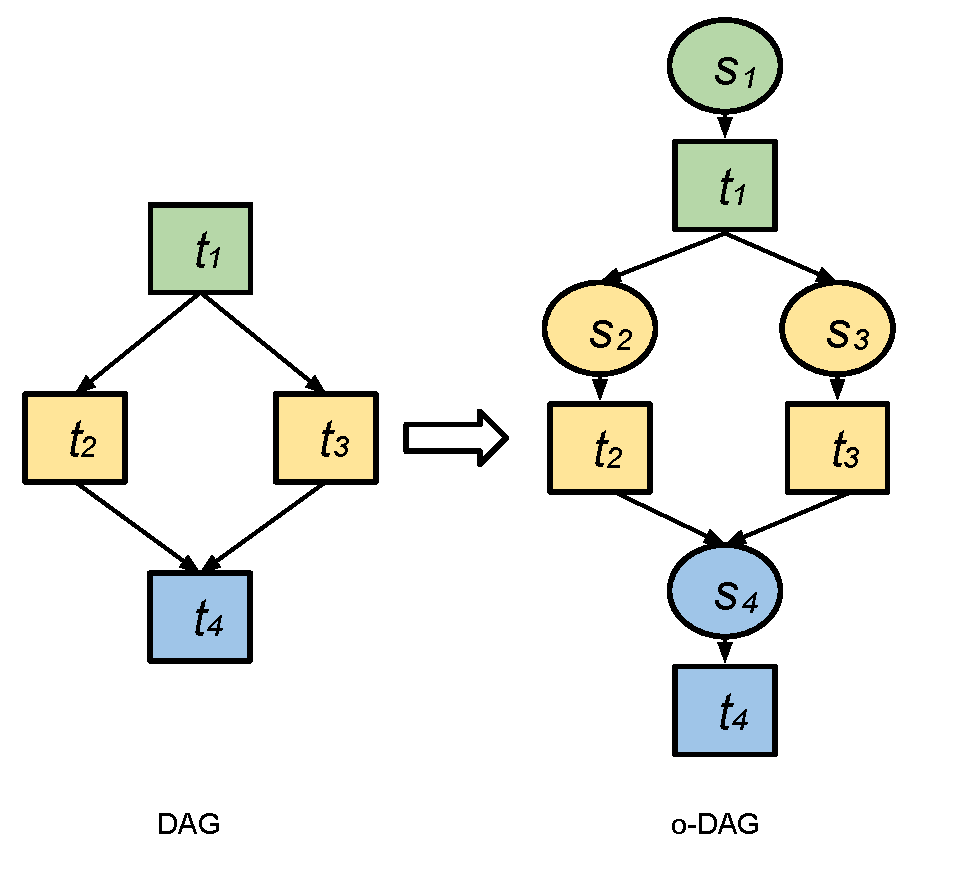
\includegraphics[width=0.6\linewidth]{figures/introduction/odag.pdf}
\centering
  \captionof{figure}{Extending DAG to o-DAG}
  \label{fig:intro_odag}
\end{figure}

Traditionally a workflow is modeled as a Directed Acyclic Graph (DAG). Each node in the DAG represents a workflow task, and the edges represent dependencies between the tasks ($t$) that constrain the order in which the tasks are executed. Each task is a program and a set of parameters that need to be executed. A job ($j$) is a single execution unit and it contains one or multiple task(s). The dependencies typically represent data flow dependencies in the application, where the output files produced by one task are needed as inputs of another task. In this work, we extend the DAG model to be overhead aware (o-DAG). The reason is that system overheads play an important role in workflow execution and they constitute a major part of the overall runtime when tasks are poorly clustered. Fig~\ref{fig:intro_odag} shows how we augment a DAG to be an o-DAG with the capability to represent scheduling overheads ($s$) such as workflow engine delay, queue delay, and postscript delay. The classification of overheads is based on the model of a typical workflow management system shown in Fig~\ref{fig:intro_system}. The components in this WMS are listed below: 

\begin{figure}[h!]
\centering
  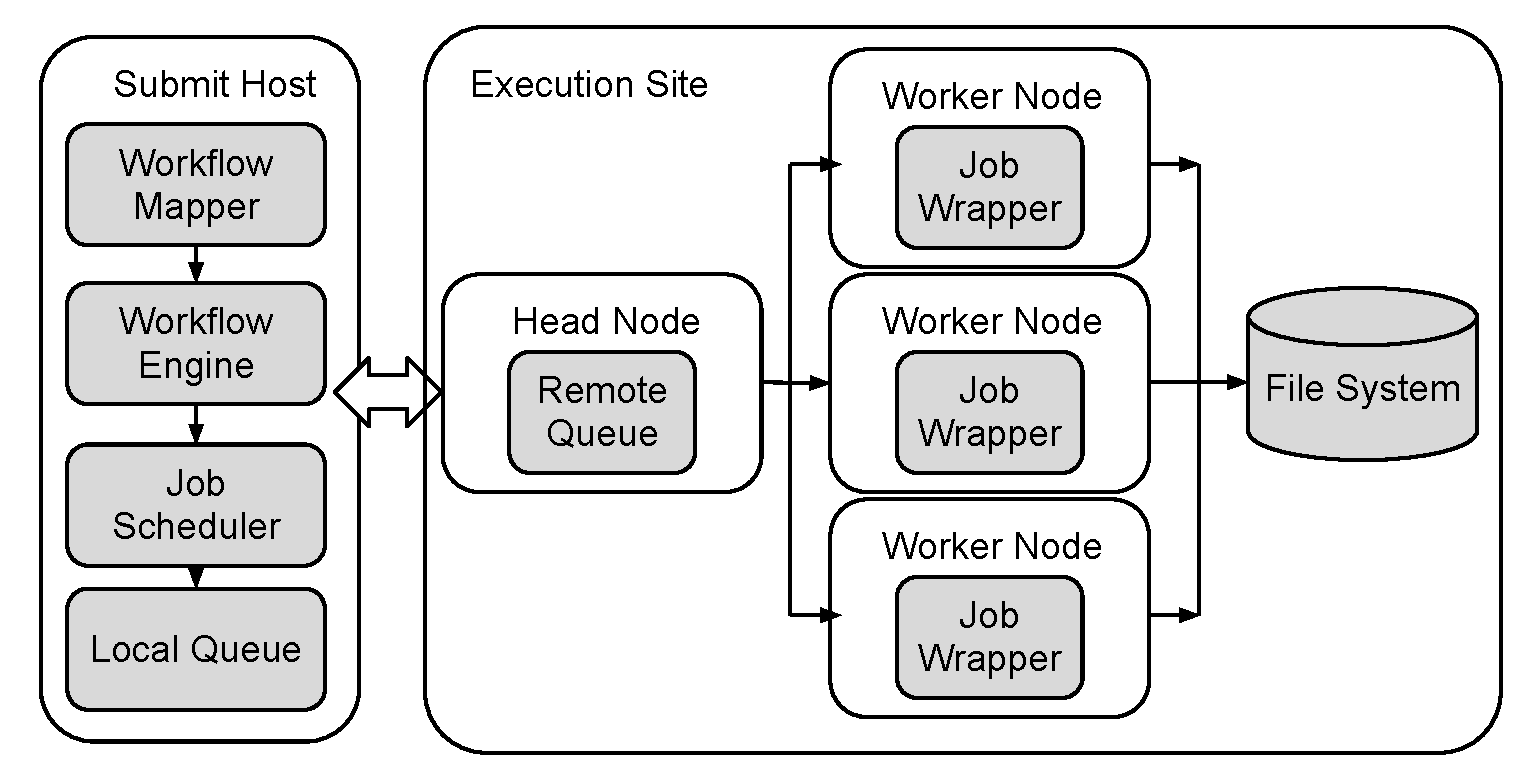
\includegraphics[width=0.7\linewidth]{figures/introduction/model.pdf}

  \caption{System Model}
  \label{fig:intro_system}
\end{figure}


\textbf{Workflow Mapper} generates an executable workflow based on an abstract workflow provided by the user or workflow composition system. 

\textbf{Workflow Engine} executes the jobs defined by the workflow in order of their dependencies. Only free jobs that have all their parent jobs completed are submitted to  Job Scheduler. 

\textbf{Job Scheduler} and \textbf{Local Queue} manage individual workflow jobs and supervise their execution on local and remote resources.

\textbf{Job Wrapper} extracts tasks from clustered jobs and executes them at the worker nodes. 


\begin{figure}[h!]
\centering
 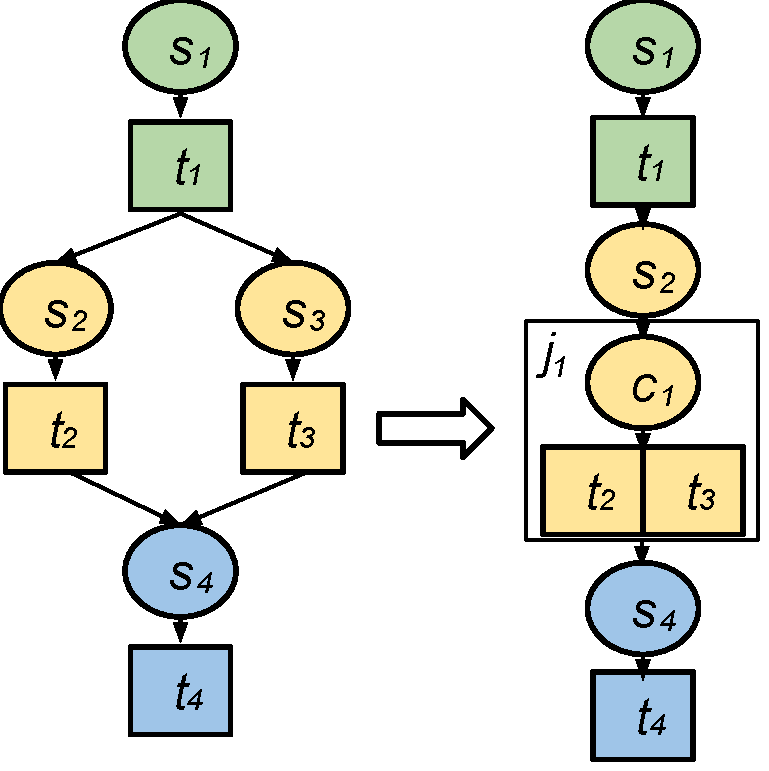
\includegraphics[width=0.5\linewidth]{figures/introduction/hc.pdf}
  \captionof{figure}{Task Clustering}
  \label{fig:intro_hc}
\end{figure}


\begin{figure}[!htb]
\centering
 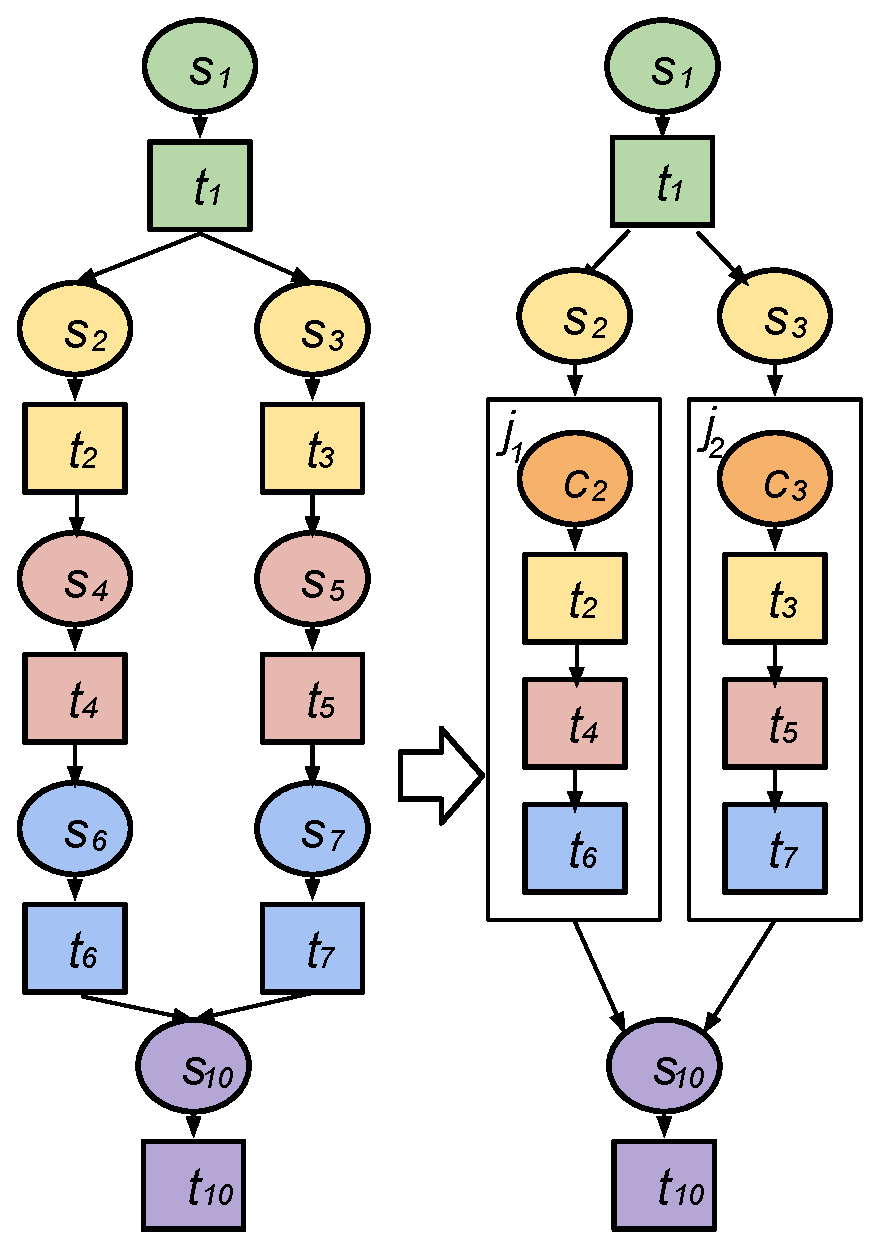
\includegraphics[width=0.5\linewidth]{figures/model/vc.pdf}
  \captionof{figure}{An example of vertical clustering.}
  \label{fig:model_vc}
\end{figure}

%Clustering delay ($c$) measures the difference between the sum of the actual task runtime and the job runtime seen by the job scheduler. The cause of clustering delay is usually the use of a job wrapper to execute a clustered job. 
%The job wrapper takes some time to extract the list of tasks and to launch them.

%With o-DAG model, we can explicitly express the process of task clustering. For example, in Fig~\ref{fig:intro_hc}, two tasks $t_2$ and $t_3$ without data dependency between them are merged into a clustered job $j_1$. Scheduling overheads ($s_3$) are reduced but clustering delay ($c_1$) is added. 

With an o-DAG model, we can explicitly express the process of task clustering. In this paper, we address task clustering horizontally and vertically. \textbf{Horizontal Clustering} (HC) merges multiple tasks that are at the same horizontal level of the workflow, in which the horizontal level of a task is defined as the longest distance from the entry task of the DAG to this task. \textbf{Vertical Clustering} (VC) merges tasks within a pipeline of the workflow. Tasks at the same pipeline share a single-parent-single-child relationship, which means a task $t_a$ is the unique parent of a task $t_b$, which is the unique child of $t_a$. 


Figure~\ref{fig:intro_hc} shows a simple example of how to perform HC, in which two tasks $t_2$ and $t_3$, without a data dependency between them, are merged into a clustered job $j_1$. A job is a single execution unit composed by one or multiple task(s). Job wrappers are commonly used to execute clustered jobs, but they add an overhead denoted by the clustering delay $c$. The clustering delay measures the difference between the sum of the actual task runtimes and the job runtime seen by the job scheduler. 
After horizontal clustering, $t_2$ and $t_3$ in $j_1$ can be executed in sequence or in parallel, if parallelism in one compute node is supported. In this work, we consider sequential executions only. Given a single resource, the overall runtime for the workflow in Figure~\ref{fig:intro_hc} (left) is $runtime_l= \sum_{i=1}^{4}(s_i+t_i)$, and the overall runtime for the clustered workflow in Figure~\ref{fig:intro_hc} (right) is $runtime_r=s_1+t_1+s_2+c_1+t_2+t_3+s_4+t_4$.  $runtime_l > runtime_r$ as long as $c_1 < s_3$, which is often the case in many distributed systems since the clustering delay within a single execution node is usually shorter than the scheduling overhead across different execution nodes. 


Figure~\ref{fig:model_vc} illustrates an example of vertical clustering, in which tasks $t_2$, $t_4$, and $t_6$ are merged into $j_1$, while tasks $t_3$, $t_5$, and $t_7$ are merged into $j_2$. Similarly, clustering delays $c_2$ and $c_3$ are added to $j_1$ and $j_2$ respectively, but system overheads $s_4$, $s_5$, $s_6$, and $s_7$ are removed. 







%Traditionally the optimization of workflow performance has been focusing on reducing overall runtime of computational activities through techniques such as  task scheduling that aims to adjust the mapping from tasks to resources. However, these approaches have over-simplified the characteristics of real distributed environments and under-estimated the complexity of large scale workflows. In practice, due to the distributed nature of these resources, the large number of tasks in a workflow, and the complex dependencies among the tasks, significant system overheads can occur during workflow execution. For example, a Montage workflow has around 10,000 tasks, which is a significant load for workflow management tools to schedule or maintain. On one hand, the duration of these tasks is usually around a few seconds, but the system overheads in distributed systems such as Grids can reach up to a few minutes. Merging these short workflow tasks into a larger group of tasks and executing them together can reduce the number of operations (such as job submission) and thus reduce the system overheads significantly. The process of merging tasks into a single job (group of tasks) is called task clustering. 




%\section{Related Work}

%The Directed Acyclic Graph (DAG) has been widely used in many workflow management systems such as DAGMan \cite{DAGMan}, Pegasus \cite{Deelman2004}, Triana \cite{Taylor2006}, DAGuE \cite{Bosilca2011} and GrADS \cite{Cooper2004} . Each node in the DAG represents a workflow task, and the edges represent dependencies between the tasks that constrain the order in which the tasks are executed.  The Directed Acyclic Graph Manager (DAG-Man) \cite{DAGMan} is a service provided by Condor \cite{Frey2002} for executing multiple jobs with dependencies. The DAGMan meta-scheduler processes the DAG dynamically, by sending to the Condor scheduler the jobs as soon as their dependencies are satisfied and they become ready to execute. DAGMan can also help with the resubmission of uncompleted portions of a DAG when one or more nodes resulted in failure, which is called job retry. Pegasus \cite{Deelman2004}, which stands for Planning for Execution in Grids, was developed at the USC Information Sciences Institute as part of the GriPhyN \cite{Deelman2002} and SCEC/IT \cite{Maechling2007} projects. Pegasus receives an abstract workflow description in a XML format from users, produces a concrete or executable workflow, and submits it to DAGMan for execution. 

%A Petri net is a directed bipartite graph, in which the nodes represent transitions and places. The directed arcs describe which places are pre- and/or postconditions for which transitions occurs. Ordinary Petri nets and their extensions have been widely used for the specification, analysis and implementation of workflows \cite{Aalst1998}. Petri nets also enable powerful analysis techniques, which can be used to verify the correctness of workflow procedures. In the scientific workflow community, Petri nets have also been utilized and GWorkflowDL \cite{Vossberg2008}, Grid-Flow \cite{Guan2004} and FlowManager \cite{Aversano2002} are representative examples of this. 

%ASKALON \cite{Fahringer2005} is a Grid environment for composition and execution of scientific workflow applications and uses the standard Web Services Description Language (WSDL) to model workflows. WSDL is an XML format for describing network services as a set of endpoints operating on messages containing either document-oriented or procedure-oriented information. The operations and messages are described abstractly, and then bound to a concrete network protocol and message format to define an endpoint. In ASKALON, the scheduler optimizes the workflow performance using the execution time as the most important goal function. The scheduler interacts with the enactment engine, which is a service that supervises the reliable and fault tolerant execution of the tasks and the transfer of files. 
 
%Compared to these approaches, we extend the original DAG model to be overhead aware so as to analyze the performance of task clustering. An overhead \cite{Prodan2008, Prodan2007} is defined as the time of performing miscellaneous work other than executing the user’s computational activities. In our overhead-aware DAG model (o-DAG), a node can represent either a computational task/job or system overhead during the runtime. A directed edge can represent either a data dependencies between computational tasks/jobs or a control dependency between overheads and computations. Such an extension of the DAG model provides us the ability to model the process of task clustering and analyze the runtime performance of different task clustering strategies. 

%Overheads play an important role in distributed systems. Stratan et al. \cite{Stratan2008} evaluates workflow engines including DAGMan/Condor and Karajan/Globus in a real-world grid environment. Their methodology focuses on five system characteristics: the overhead, the raw performance, the stability, the scalability and the reliability. They have pointed out that head node consumption should not be negligible and the main bottleneck in a busy system is often the head node. Prodan et al. \cite{Prodan2008} offers a complete grid workflow overhead classification and a systematic measurement of overheads. Östberg et al. \cite{Östberg2011} used the Grid Job Management Framework (GJMF) as a testbed for characterization of Grid Service-Oriented Architecture overhead, and evaluate the efficiency of a set of design patterns for overhead mediation mechanisms featured in the framework. In comparison with their work, (1) we focus on measuring the overlap of major overheads imposed by workflow management systems and execution environments; (2) we present a study of the distribution of overheads instead of just overall numbers; (3) we compare workflows running in different platforms (dedicated clusters, clouds, grids) and different environments (resource availability, file systems), explaining how they influence the resulting overheads; and (4) we analyze how existing optimization techniques improve the workflow runtime by reducing or overlapping overheads.


%Fragmentation \cite{Rodríguez2012} is a well known effect in resource allocation, which decreases the resource utilization, as studied in \cite{Smith2000}. Whenever a resource allocation fails, even though enough free capacity is available, fragmentation is easily spotted as cause. In \cite{Gehr2009}, a new way for measuring the fragmentation of a system, as well as their correlation with jobs rejection, is presented. It shows that the proposed fragmentation measure is a good indicator of the state of the system. In this work, we are also interested in the resource under-utilization problem and we use a few cumulative metrics to measure the fragmentation. 


%Performance Analysis of scientific workflows has also been studied in \cite{Rubing2009, Calasanz2008, Truong2004, Uysal1998}. The performance method proposed by Duan et al. \cite{Rubing2009} is based on a hybrid Bayesian-neural network for predicting the execution time of workflow tasks. Bayesian network is a graphical modeling approach that we use to model the effects of different factors affecting the execution time (referred as factors or variables), and the interdependence of the factors among each other. The important attributes are dynamically selected by the Bayesian network and fed into a radial basis function neural network to make further predictions. In comparison, our work in overhead analysis focuses on the relationship between system overheads and the performance of different optimization methods. We investigated a wide range of scientific workflows and analyzed how system overheads influence the performance of optimization of these workflows. 


%Because in Grid systems communication delays are significant all algorithms must achieve maximum parallelism while minimizing data communication. 

%Task Clustering reduces the communication cost and scheduling overheads by grouping the heavily communicating tasks or short runtime tasks to the same job and then assigning the job in a cluster to the same resources. 
%Task clustering algorithms can have two phases: the initial task clustering and a post-clustering phase which can refine the clusters produced in the previous phase. Our work has covered both phases. 

%The low performance of lightweight (a.k.a. fine-grained) tasks is a common problem on widely distributed platforms where the communication overheads and scheduling overheads are high, such as grid systems. To address this issue, fine-grained tasks are commonly merged into coarse-grained tasks \cite{Muthuvelu2005, Muthuvelu2013, Keat2006}, which reduces the cost of data transfers when grouped tasks share input data \cite{Muthuvelu2005} and saves scheduling overheads such as queueing time when resources are limited. However, task grouping also limits parallelism and therefore should be used carefully. Muthuvelu et al. \cite{Muthuvelu2013} proposed an algorithm to group bag of tasks based on their granularity size defined as the processing time of the task on the resource. Resources are ordered by their decreasing values of capacity (in MIPS) and tasks are grouped up to the resource capacity. Then, Keat et al. \cite{Keat2006} and Ang et al. \cite{Ang2009} extended the work of Muthuvelu et al. by introducing bandwidth to enhance the performance of task clustering. Resources are sorted in descending order of bandwidth, then assigned to grouped tasks downward ordered by processing requirement length. Afterwards, Soni et al. \cite{Soni2010} proposed an algorithm to group lightweight tasks into coarse-grained tasks (GBJS) based on processing capability, bandwidth, and memory-size of the available resources. Tasks are sorted into ascending order of required computational power, then, selected in first come first serve order to be grouped according to the capability of the resources. Zomaya and Chan \cite{Zomaya2004} studied limitations and ideal control parameters of task clustering by using genetic algorithm. Their algorithm performs task selection based on the earliest task start time and task communication costs; it converges to an optimal solution of the number of clustered jobs and tasks per clustered job. In contrast, our work has discussed the influence of data dependencies across different levels while they only focus on computational activities (bag-of-tasks). 


%Singh \cite{Singh2008} proposed to use horizontal clustering and label based clustering in scientific workflows to reduce the scheduling overheads in a best-effort approach. The horizontal clustering merges tasks at the same level, while level of a task refers to the distance from a root task to this task using Breadth-First-Search. Label based clustering uses labels set by the users manually and merges tasks with the same labels together. Task clustering strategies have demonstrated their effect in some scientific workflows \cite{Rynge2012, Maheshwari2012, Hussin2010, Liu2009}.  Li \cite{Li2011}  developed algorithm that uses horizontal clustering to group tasks that can be scheduled to run simultaneously. Tasks with the same scheduling priority (determined by the scheduling level) are merged and scheduled to run simultaneously. Cao et al. \cite{Cao2008} proposed a static scheduling heuristic, called DAGMap that consists of three phases, namely prioritizing, grouping, and independent task scheduling. Task grouping is based on dependency relationships and task upward priority (the longest distance form this task to the exit task). Compared to their work, we propose a generic workflow model that takes system overheads into consideration and provide a series of overhead aware task clustering strategies to optimize the overall runtime performance of workflows. 

%Task clustering is one typical category of task scheduling, which maps resources to tasks based on different criteria. List Heuristics assign a priority to a task and the scheduling algorithms attempt to execute the higher priority nodes first. Most scheduling algorithms for Grid systems are based on this approach. For example, scheduling algorithms, such as HEFT \cite{Topcuoglu2002}, MaxMin \cite{Braun2001}, MinMin \cite{Blythe2005}, etc., have been widely used in optimizing the runtime performance of many scientific workflows. Genetic Algorithms \cite{Adamuthe2011} and Neural Network \cite{Babu2012} are also proposed to address the scheduling problem. Compared to them, we aim to generate a group of tasks that are suitable for scheduling and execution while the resource selection is not our major challenge since we already have many mature scheduling algorithms. 




%Pandey et al. (2009) used task clustering to schedule data-intensive tasks for a medical application workflow. They clustered tasks based on their execution time, data transfer and level. If tasks were having high deviation and value of average execution time, they were executed without clustering. Tasks with lower deviation and value of execution time were clustered together. They showed that clustering tasks for data-intensive application workflows has better makespan than scheduling the workflow without clustering, mainly attributed to the decrease in file transfers between tasks in the same cluster.



%Traditionally a workflow is modeled as a Directed Acyclic Graph (DAG). Each node in the DAG represents a workflow task, and the edges represent dependencies between the tasks ($t$) that constrain the order in which the tasks are executed. Each task is a program and a set of parameters that need to be executed. Fig~\ref{fig:intro_odag} (left) shows a simple workflow with four tasks. A job ($j$) is a single execution unit and it contains one or multiple task(s). The dependencies typically represent data flow dependencies in the application, where the output files produced by one task are needed as inputs of another task. 
%In this paper, we extend the DAG model to be overhead aware (o-DAG). The reason is that system overheads play an important role in workflow execution and they constitute a major part of the overall runtime when tasks are poorly clustered. 
%Fig~\ref{fig:intro_odag} (right) shows how we augment a DAG in Fig~\ref{fig:intro_odag} (left) to be an o-DAG with the capability to represent scheduling overheads ($s$) such as workflow engine delay ($w$), queue delay ($q$), and postscript delay ($q$). Fig~\ref{fig:intro_hc} further shows how we perform task clustering in this simple workflow, in which we merge $t_1$ and $t_2$ into a new job $j_4$. The scheduling overheads associated with $t_2$ and $t_3$ are removed and the overheads including the clustering delay ($c_1$) of $j_1$ are added. 

%To execute this workflow, a workflow engine such as DAGMan \cite{DAGMan} processes this DAG starting from the root task ($t_0$) and then executes each task without violating the data dependencies. Take the example of one available resource, a possible schedule would be $t_0\rightarrow t_1\rightarrow t_2\rightarrow t_3$ or $t_0\rightarrow t_2\rightarrow t_1\rightarrow t_3$. Both of the two schedules satisfy the data dependencies are thereby they are correct. 






The classification of overheads is based on the model of a typical workflow management system (WMS) shown in Fig~\ref{fig:intro_system}. The components in this WMS are listed below: 


\textbf{Workflow Mapper} generates an executable workflow based on an abstract workflow provided by the user or a workflow composition system. 

\textbf{Workflow Engine} executes the jobs in order of their dependencies. Only free jobs that have all their parent jobs completed are submitted to  Job Scheduler. 

\textbf{Job Scheduler} and \textbf{Local Queue} manage individual workflow jobs and supervise their execution on local and remote resources.

\textbf{Job Wrapper} extracts tasks from clustered jobs and executes them at the worker nodes. 





%An overhead is defined as the time of performing miscellaneous work other than executing the user’s computational activities. 
%The execution of scientific workflows often suffers from a variety of overheads in the distributed environment. 
%Due to the distributed nature of these resources, the large number of tasks in a workflow, and the complex dependencies among the tasks, significant overheads can occur during the workflow execution. 
%It is essential to identify the different overheads and to evaluate how different optimization methods reduce overheads and improve runtime performance. 
%In this section, we present an overhead analysis for a set of workflows run on cloud, grid, or cluster platforms. 
%We present the overhead distributions and the patterns that they have performed. 

\section{Workflow Overheads}
\subsection{Overhead Classification}


\begin{figure}[h!]
	\centering
    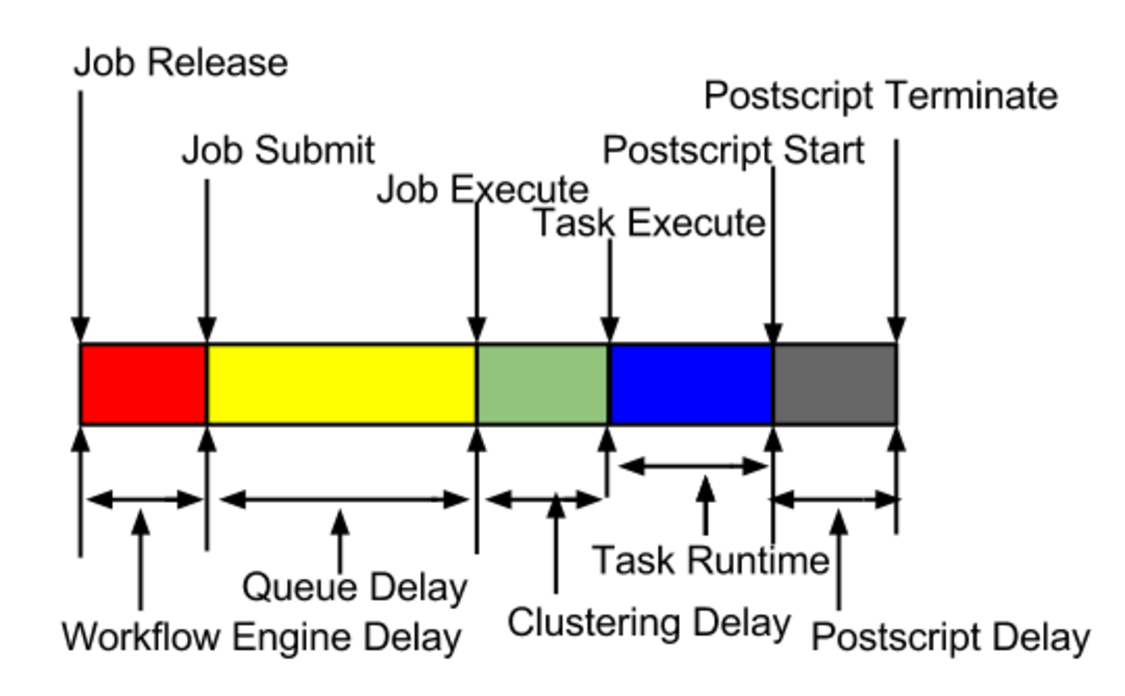
\includegraphics[width=0.7\textwidth]{figures/model/overhead.pdf}
    \caption{Workflow Events}
    \label{fig:model_overhead}
\end{figure}


The execution of a job is comprised of a series of events as shown in Figure~\ref{fig:model_overhead} and they are defined as:
\begin{enumerate}
\item Job Release is defined as the time when the workflow engine identifies that a job is ready to be submitted (when its parents have successfully completed). 
\item Job Submit is defined as the time when the workflow engine submits a job to the local queue. 
\item Job Execute is defined as the time when the workflow engine sees a job is being executed. 
\item Task Execute is defined as the time when the job wrapper sees a task is being executed. 

\item Postscript Start is defined as the time when the workflow engine starts to execute a postscript. 
\item Postscript Terminate is defined as the time when the postscript returns a status code (success or failure). 
\end{enumerate}

Figure~\ref{fig:model_overhead} shows a typical timeline of overheads and runtime in a compute job. We do not specify the data transfer delay in this timeline because data transfer is handled by data transfer jobs (stage-in and stage-out jobs). 

We have classified workflow overheads into five categories as follows. 
\begin{enumerate}

\item{Workflow Engine Delay} measures the time between when the last parent job of a job completes and the time when the job gets submitted to the local queue. 
%In case of retries the value of the last retry is used for the calculation. 
The completion time of the last parent job means this job is released to the ready queue and is waiting for resources to be assigned to it. The workflow engine delay reflects the efficiency of a workflow engine (i.e., DAGMan \cite{DAGMan}). 

\item{Queue Delay} is defined as the time between the submission of a job by the workflow engine to the local queue and the time the local scheduler sees the job running. This overhead reflects the efficiency of the local workflow scheduler (e.g. Condor \cite{Frey2002}) to execute a job and the availability of resources for the execution of this job. 
%The queue delay is an estimate of the time spent in the local queue on the submit host. 

\item{Postscript Delay } is the time taken to execute a lightweight script under some execution systems after the execution of a job. Postscripts examine the status code of a job after the computational part of this job is done.

%\item{Data Transfer Delay} happens when data is transferred between nodes. It includes three different types of processes: staging data in, cleaning up, and staging data out. Stage-in jobs transfer input files from source sites to execution sites before the computation starts. Cleanup jobs delete intermediate data that is no longer needed by the remainder of the workflow. Stage-out jobs transfer workflow output data to archiving sites for storage and analysis.

\item{Clustering Delay} measures the difference between the sum of the actual task runtime and the job runtime seen by the job wrapper. The cause of Clustering Delay is usually because we use a job wrapper in worker nodes to execute a clustered job that requires some delay to extract the list of tasks. 
\end{enumerate}

\subsection{Overhead Distribution}

%We examined the overhead distributions of a wide range of workflows in our experiments . These workflows were run on distributed platforms including clouds, grids and dedicated clusters. 
%%On clouds, virtual machines were provisioned and then the required services (such as file transfer services) were deployed. 
%We examined two clouds: Amazon EC2 \cite{AmazonEC2}  and FutureGrid \cite{FutureGrid}. Amazon EC2 is a commercial, public cloud that is been widely used in distributed computing. 
We examined the overhead distributions of a widely used astronomy workflow called Montage \cite{Berriman2004} that is used to construct large image mosaics of the sky. Montage was run on FutureGrid \cite{FutureGrid}. FutureGrid is a distributed, high-performance testbed that provides scientists with a set of computing resources to develop parallel, grid, and cloud applications. 
%%On grids, grid resources were provisioned through Corral \cite{Juve2010a} and the required services were already installed before execution. A grid site may be a cluster system or a heterogeneous and dynamic collection of machines. In a dedicated cluster, Condor was used to schedule jobs directly to worker nodes. Part of this experimental data (especially those workflows run on Amazon EC2) has been studied in \cite{Juve2010c} but without a detailed overhead analysis. 
%For the Amazon EC2 experiments, the performance with different numbers of resources and file system types is compared.
%The workflows and execution environments we examined include:
%\begin{enumerate}
%%\item Epigenomics \cite{Epigenome} maps short DNA segments collected with high-throughput gene sequencing machines to a reference genome. It was run on Amazon EC2. 

%%\item Proteomics \cite{Proteomics} is an application developed by scientists at Ohio State University and it is used for mass-spectrometry-based proteomics. It was run on Amazon EC2. 

%\item Broadband \cite{Graves2008} is an application that enables researchers to combine long-period deterministic seismograms with high-frequency stochastic seismograms. It was run on Amazon EC2. 

%\item Montage \cite{Berriman2004} is an astronomy application used to construct large image mosaics of the sky. The Montage workflows were run on FutureGrid.

%\item CyberShake \cite{Graves2010, Callaghan2008, Deelman2006} is a seismology application that calculates Probabilistic Seismic Hazard curves for geographic sites in the Southern California region. It was run on the HPCC cluster \cite{HPCC} at the University of Southern California. 

%\item SIPHT \cite{Livny2008} conducts searches for small untranslated RNAs (sRNAs) that are used to regulate essential biochemical processes in bacteria. It was run on a Condor cluster at the University of Wisconsin at Madison. 

%\item LIGO \cite{Abramovici1992,LIGO} workflows are used to search for gravitational wave signatures in data collected by large-scale interferometers. We present one partition of the entire workflow in this work. It was run on a local cluster at the Syracuse University.
%\end{enumerate}
%
%\begin{figure}[h!]
%	\centering
%    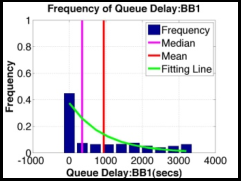
\includegraphics[width=0.4\textwidth]{figures/model/BB1.pdf}
%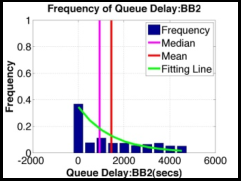
\includegraphics[width=0.4\textwidth]{figures/model/BB2.pdf}
%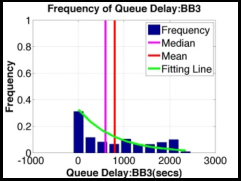
\includegraphics[width=0.4\textwidth]{figures/model/BB3.pdf}
%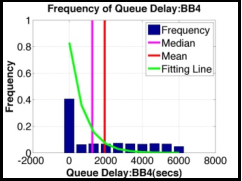
\includegraphics[width=0.4\textwidth]{figures/model/BB4.pdf}
%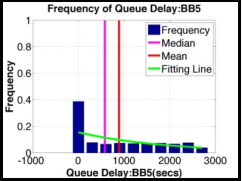
\includegraphics[width=0.4\textwidth]{figures/model/BB5.pdf}
%    \caption{Frequency Distribution of Queue Delay in Broadband}
%    \label{fig:model_broadband_distribution}
%\end{figure}
%
%\begin{table}[h!]
%\caption{Makespan of Broadband}
%\label{tab:model_broadband}
%\centering
%\begin{tabular}{lrrrr}
%\hline
%     &      Makespan &     Num of Nodes &    File System  \\
%\hline
%BB1 & 1:08:17 & 8 & NFS\\
%BB2 & 1:29:23 & 4 & NFS \\
%BB3 & 1:32:57 & 4 & PVFS \\
%BB4 & 1:51:14 & 1 & NFS \\
%BB5 & 0:52:48 & 1 & shm \\
%\hline
%\end{tabular}
%\end{table} 
%
%\begin{table}[h!]
%\caption{the SSE (sum of squares of error) of different fitting distribution}
%\label{tab:model_broadband_sse}
%\centering
%\begin{tabular}{lrrrr}
%\hline
%SSE(Unit: $10^4$)     &      Exponential &  Gamma & Normal & Weibull \\
%\hline
%BB1 & 3.57 & 232 & 8.69 & 235.2\\
%BB2 & 2.33 & 244 & 5.59 & 181.0\\
%BB3 & 1.97 & 73.9 & 4.18 & 52.4\\
%BB4 & 3.31 & 340 & 7.22 & 251.7\\
%BB5 & 2.84 & 73.1 & 6.48 & 55.4 \\
%\hline
%\end{tabular}
%\end{table} 
%
%\begin{table}[h!]
%\caption{the $\mu$ of the exponential fitting distribution}
%\label{tab:model_broadband_mu}
%\centering
%\begin{tabular}{lrrrr}
%\hline
%(Unit: sec)     &      $\mu$ \\
%\hline
%BB1 & 944.85\\
%BB2 & 1451.88\\
%BB3 & 796.90\\
%BB4 & 1952.71\\
%BB5 & 892.16 \\
%\hline
%\end{tabular}
%\end{table} 
%
%\begin{table}[h!]
%\caption{the log likelihood of different fitting distribution}
%\label{tab:model_broadband_log}
%\centering
%\begin{tabular}{lrrrr}
%\hline
%Log Likelihood     &      Exponential &  Gamma & Normal & Weibull \\
%\hline
%BB1 & -6045.3 & -5802.3 & -6464.1 & -5819.6\\
%BB2 & -6376.1 & -6203.1 & -6707.9 & -6232.9\\
%BB3 & -5914.2 & -5796.4 & -6181.4 & -5825.9\\
%BB4 & -6376.1 & -6203.1 & -6707.9 & -6232.9\\
%BB5 & -6001.1 & -5891.9 & -6327.9 & -5908.1 \\
%\hline
%\end{tabular}
%\end{table} 
%
%Frequency distribution analysis serves as an important supplement to the understanding of how different execution environments influence the overheads. Figure~\ref{fig:model_broadband_distribution} presents the mean, median and the exponential fitting lines of Queue Delay in Broadband of five runs (BB1$\sim$BB5). The Broadband workflows were executed in environments with different number of worker nodes and file systems. These runs had the same jobs and used the same type of virtual machines (c1.xlarge), but they were run in different environments. The number of worker nodes was ranging from 1 to 8 and the file systems included NFS \cite{Sandberg1985}, PVFS \cite{Carns2000} and a shared memory system (shm) on a single host. 
%
%Comparing BB1, BB2 and BB4 we conclude that resource availability influences the distribution of the queue delay. Although for all the five runs, most of the queue delays (30\%$\sim$40\%) last less than 50 seconds, the maximum duration of queue delay increases with the decrease of resource availability. With more resources available, the local scheduler is able to find a resource for execution more quickly. BB3 is installed with PVFS, which performs worse than BB2 with NFS in this experiment. The shared memory system can also improve the performance, but it is limited to the case with only one host.  
%
%We use the Matlab Distribution Fitting tool \cite{Matlab} to analyze the distribution of the queue delay. This tool aims to maximize the log likelihood of the parameters. Table~\ref{tab:model_broadband_log} shows that the queue delay satisfies the Weibull and Gamma distribution better in terms of the log likelihood. However, Table~\ref{tab:model_broadband_sse} shows that in terms of SSE (sum of squares of error), the exponential and normal distributions perform better. For simplicity, we use an exponential distribution to describe the queue delay:
%
%\begin{equation} \label{eq:model_f1}
% \phi_1(x)=\frac{1}{\mu}e^{-\frac{x}{\mu}}\varepsilon(x)
%\end{equation}
%
%$\varepsilon(x)$ is an unit step function. The estimates of $\mu$ are listed in Table~\ref{tab:model_broadband_mu}. 

%Figure~\ref{fig:model_cybershake_distribution} shows the mean and standard deviation of all 78 partitions of the entire CyberShake workflow. The standard deviation is comparable to the mean of the overheads, which we attribute to the fact that HPCC comprises a diverse mix of computing and data resources and is shared among many users across the campus. 
Figure~\ref{fig:model_montage_queue_delay}, \ref{fig:model_montage_engine_delay} and \ref{fig:model_montage_postscript_delay} show the overhead distribution of the Montage workflow run on the FutureGrid. The postscript delay concentrates at 7 seconds, because the postscript is only used to locally check the return status of a job and is not influenced by the remote execution environment. The workflow engine delay tends to have a uniform distribution, which is because the workflow engine spends a constant amount of time to identify that the parent jobs have completed and insert a job that is ready at the end of the local queue. 
%Normally, the queue delay has only one peak such as in Figure~\ref{fig:model_broadband_distribution}. But in this experiment, 
The queue delay has three decreasing peak points at 8, 14, and 22 seconds. We believe this is because the average postscript delay is about 7 seconds (see details in Figure~\ref{fig:model_montage_queue_delay} ) and the average runtime is 1 second. The local scheduler spends about 8 seconds finding an available resource and executing a job; if there is no resource idle, it will wait another 8 seconds for the current running jobs to finish, and so on. 
%Based on Equation~\ref{eq:model_f1}, an integrated function of the queue delay can be expressed as a combination of multiple exponential distributions:
%\begin{equation} \label{eq:model_f2}
% \phi_2(x)=\sum_{i=1}^{\infty}e^{-ai}\phi_1(x-ib)
%\end{equation}
%$a$ is the attenuation coefficient of the exponential distribution and $b$ is the average distance between the peaks, namely the period. In the example of Figure~\ref{fig:model_montage_distribution}, $a\approx0.5, b\approx7$. 

%\begin{figure}[h!]
%	\centering
%    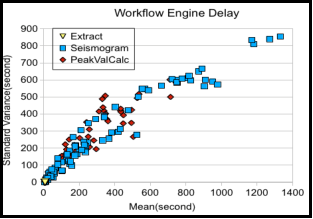
\includegraphics[height=0.3\textwidth]{figures/model/cybershake_engine_delay.pdf}
%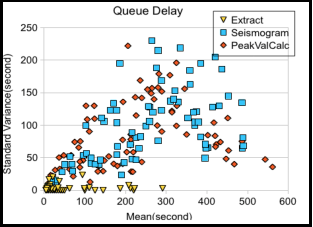
\includegraphics[height=0.3\textwidth]{figures/model/cybershake_queue_delay.pdf}
%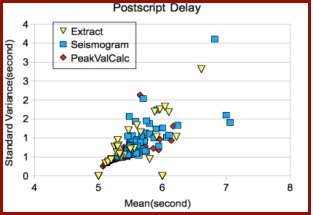
\includegraphics[width=0.4\textwidth]{figures/model/cybershake_post_delay.pdf}
%
%    \caption{Mean and Variance of all the 78 partitions of the CyberShake workflow}
%    \label{fig:model_cybershake_distribution}
%\end{figure}

\begin{figure}[h!]
	\centering
    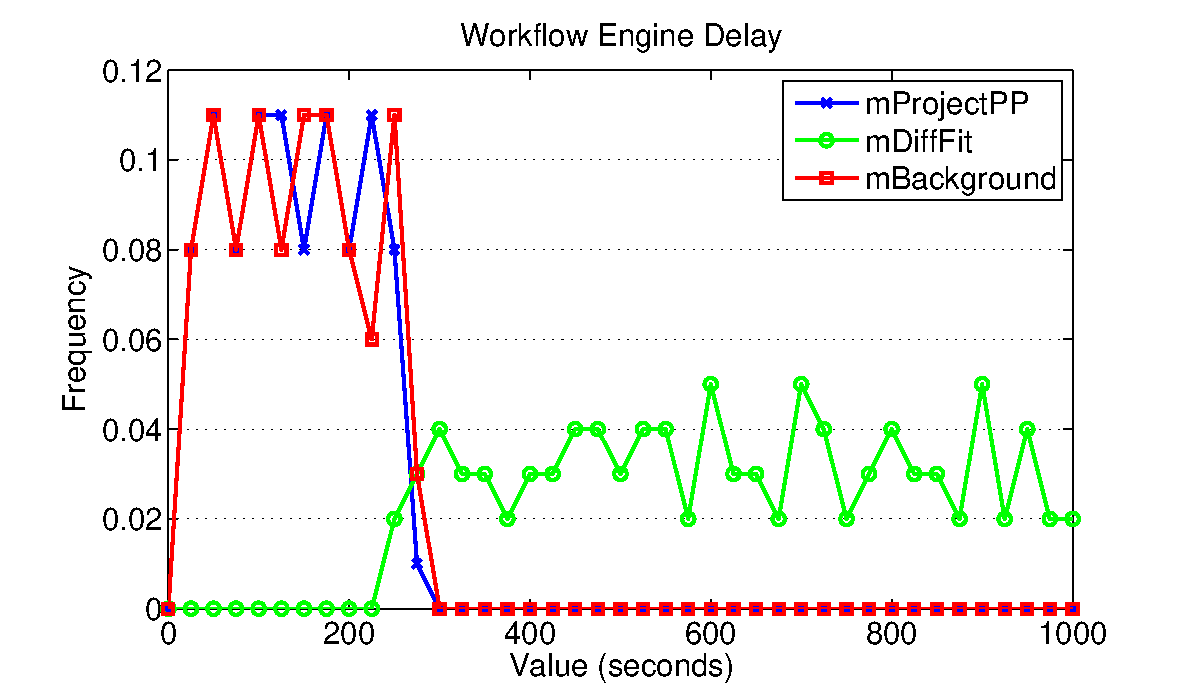
\includegraphics[height=0.5\textwidth]{figures/model/workflow_engine_delay.eps}
    \caption{Distribution of Workflow Engine Delay in the Montage workflow}
    \label{fig:model_montage_engine_delay}
\end{figure}

\begin{figure}[h!]
	\centering
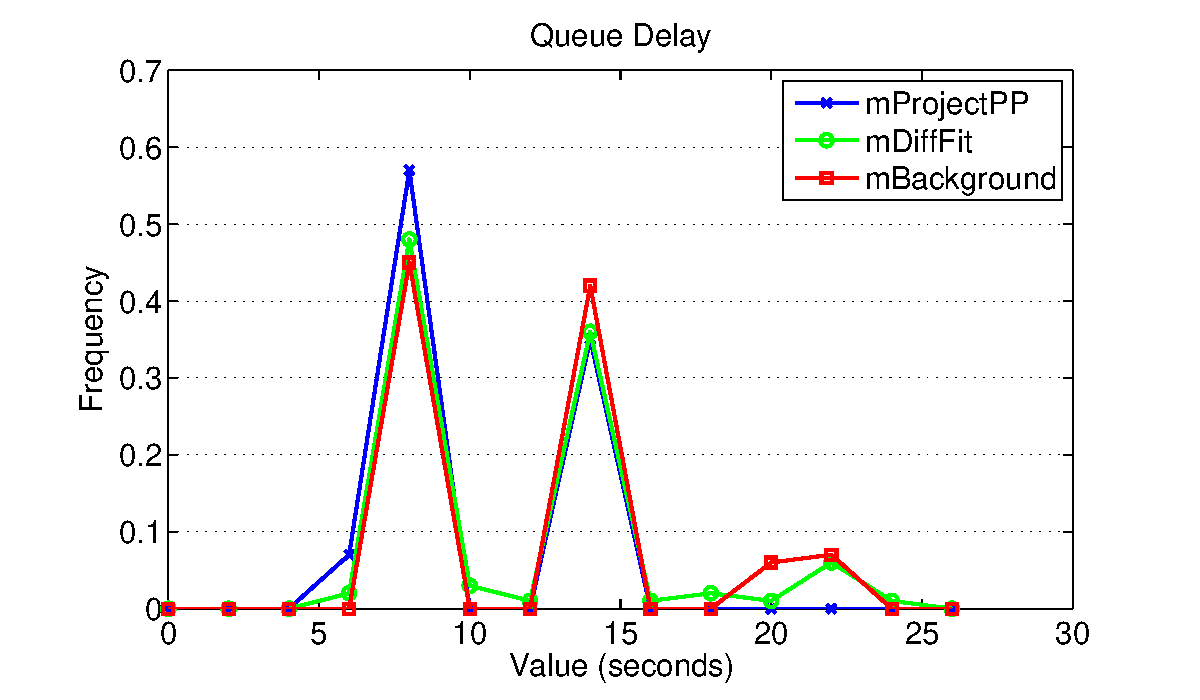
\includegraphics[height=0.5\textwidth]{figures/model/queue_delay.eps}
    \caption{Distribution of Queue Delay in the Montage workflow}
    \label{fig:model_montage_queue_delay}
\end{figure}

\begin{figure}[h!]
	\centering
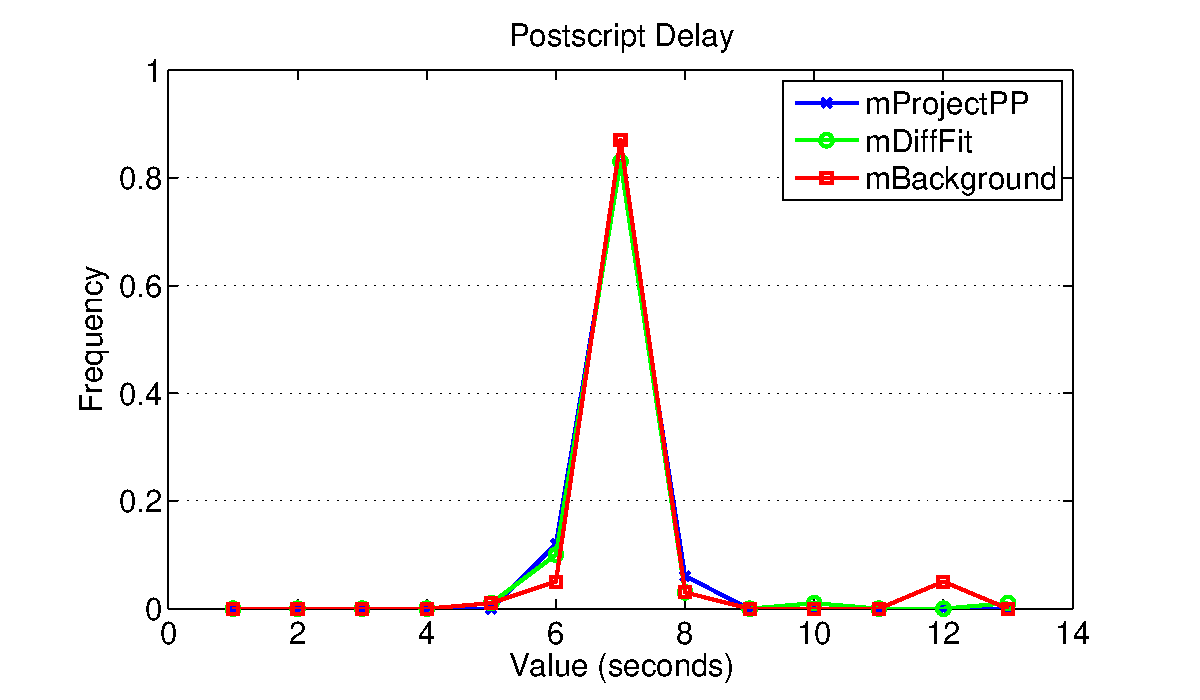
\includegraphics[width=0.9\textwidth]{figures/model/postscript_delay.eps}
    \caption{Distribution of Postscript Delay in the Montage workflow}
    \label{fig:model_montage_postscript_delay}
\end{figure}

%In our prior work \cite{Overhead2011}, we have introduced the distribution of overheads and the relationship between them. Following this, we indicate the necessity to consider the distribution of overheads rather than simply adding a constant delay after job execution. 
We use Workflow Engine Delay as an example to show the necessity to model overheads appropriately. Figure~\ref{fig:model_montage_timeline} shows a real trace of overheads and runtime in the Montage 8 degree workflow (for visibility issues, we only show the first 15 jobs at the mProjectPP level). We can see that Workflow Engine Delay increases steadily after every five jobs. For example, the Workflow Engine Delay of jobs with ID from 6 to 10 is approximately twice of that of jobs ranging from ID1 to ID5. Figure~\ref{fig:model_montage_one_run} further shows the distribution of Workflow Engine Delay of the first 20 jobs at the mProjectPP level in the Montage workflow. After every five jobs, the Workflow Engine Delay increases by 8 seconds approximately. We call this special nature of workflow overhead as cyclic increase. The reason is that Workflow Engine (in this trace it is DAGMan) releases five jobs by default in every working cycle. Therefore, simply adding a constant delay after every job execution has ignored its potential influence on the performance.

\begin{figure}[h!]
	\centering
    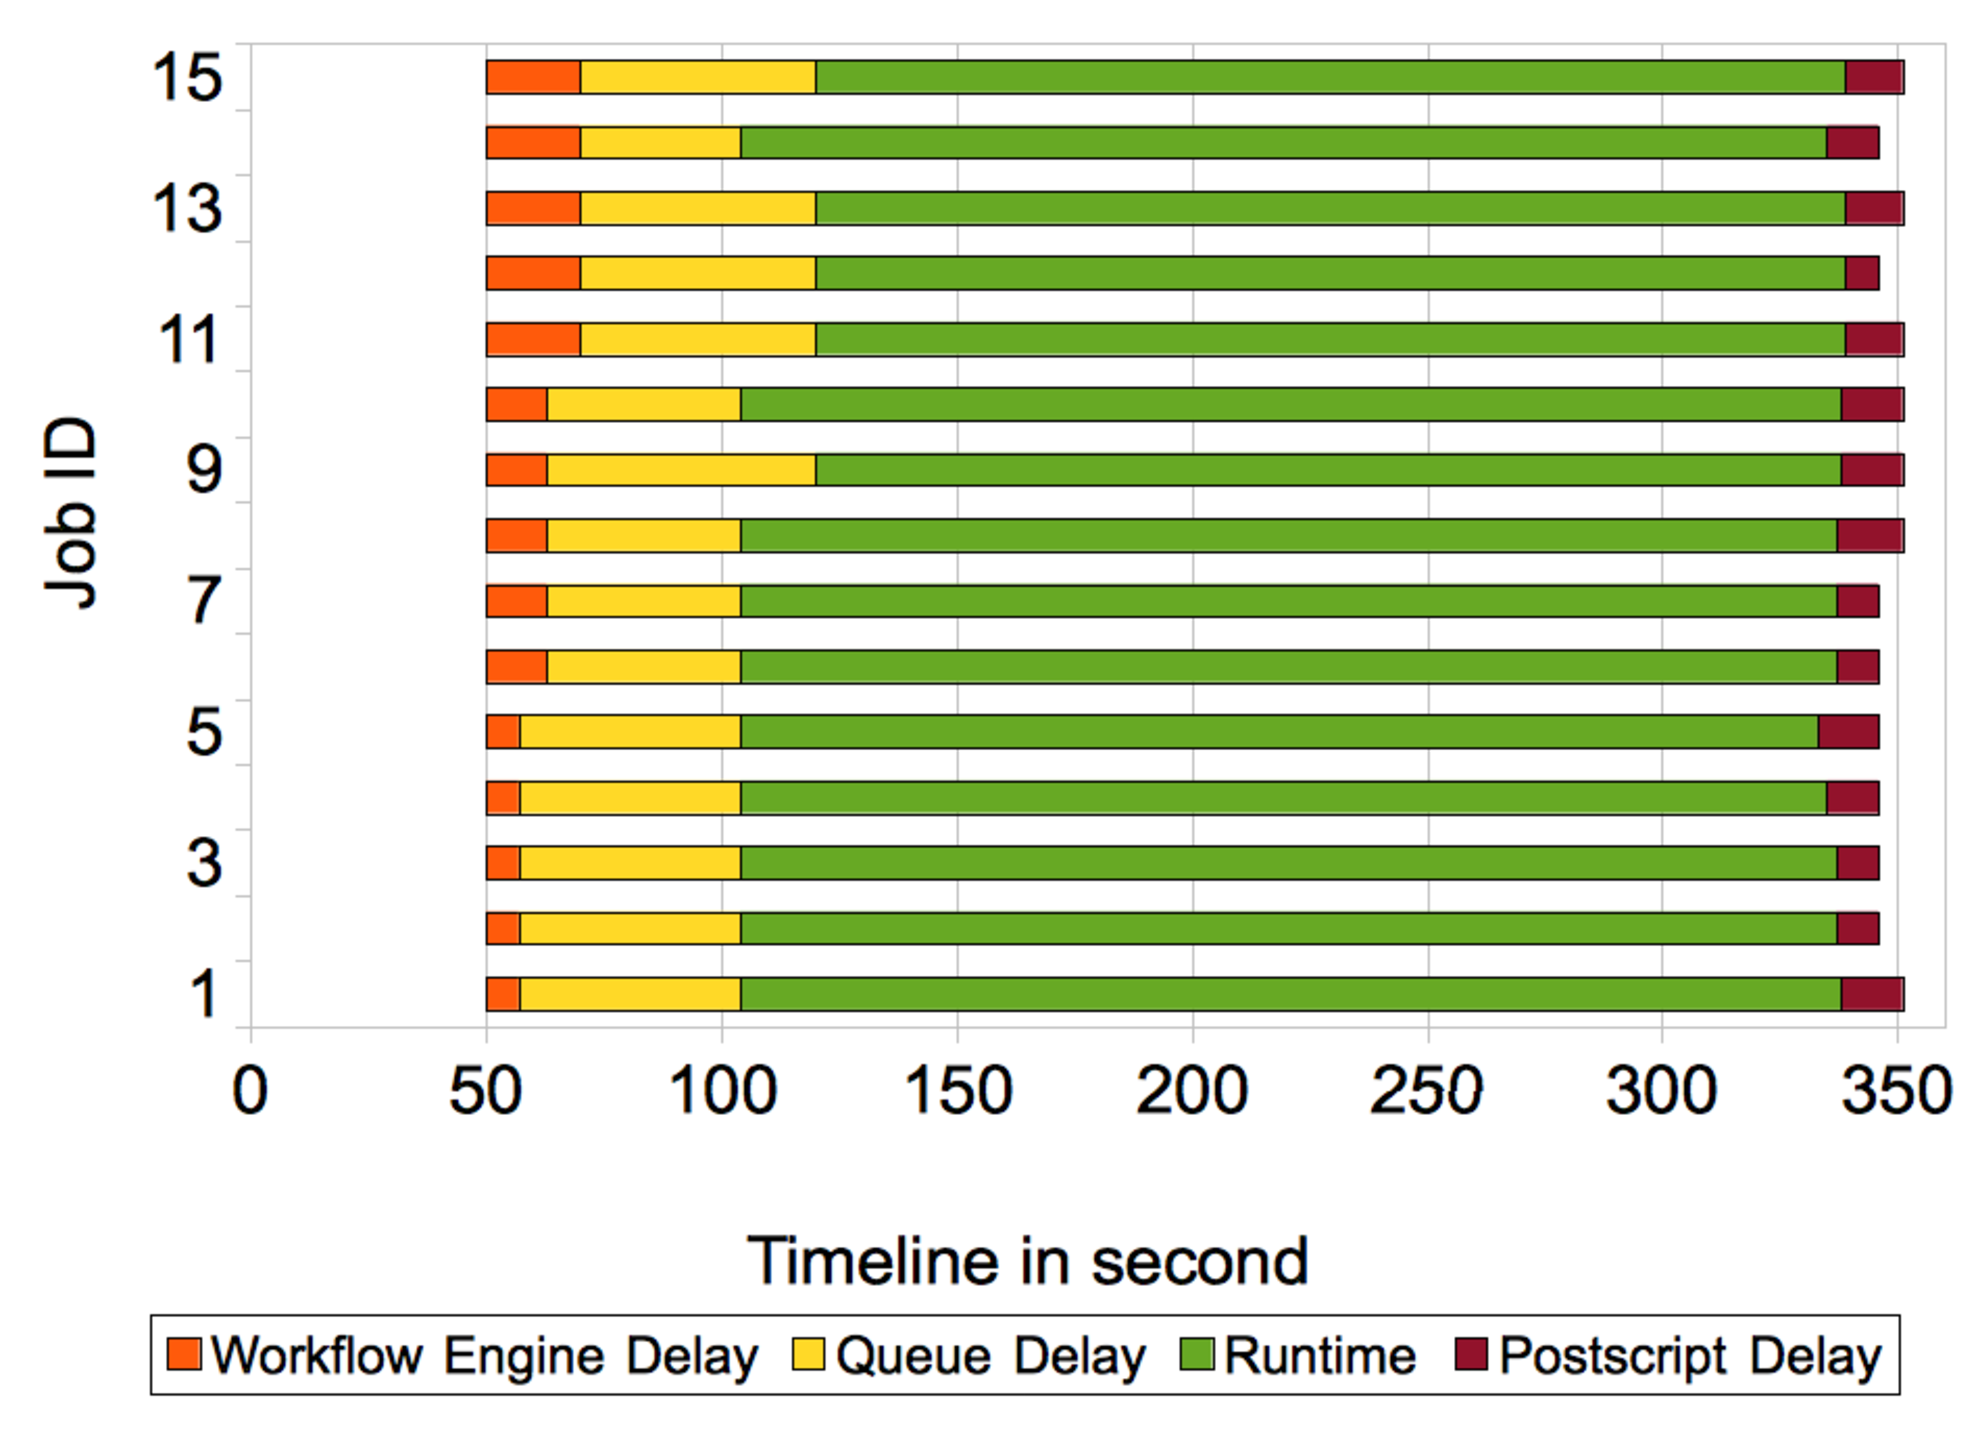
\includegraphics[width=0.7\textwidth]{figures/model/overhead_timeline2.pdf}
    \caption{Workflow Overhead and Runtime. Clustering delay and data transfer delay are not shown}
    \label{fig:model_montage_timeline}
\end{figure}




\begin{figure}

\centering
  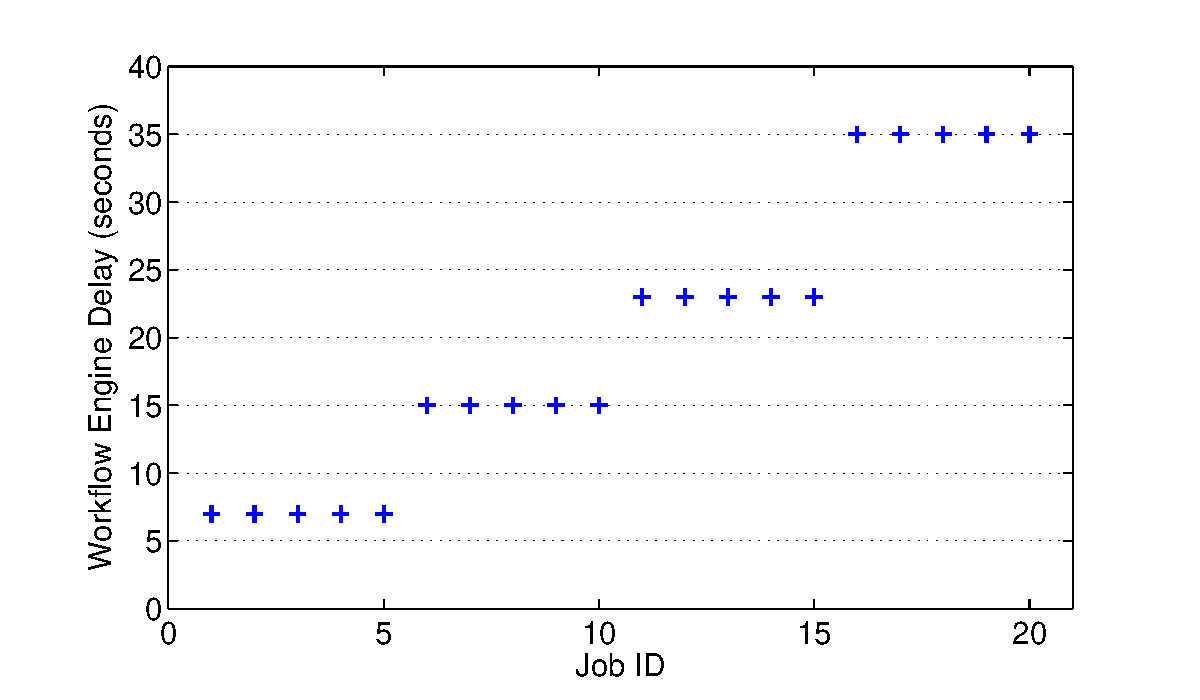
\includegraphics[width=0.9\linewidth]{figures/model/montage_one_run.eps}
    \caption{Workflow Engine Delay of mProjectPP}
    \label{fig:model_montage_one_run}
\end{figure}%
\begin{figure}
  \centering
  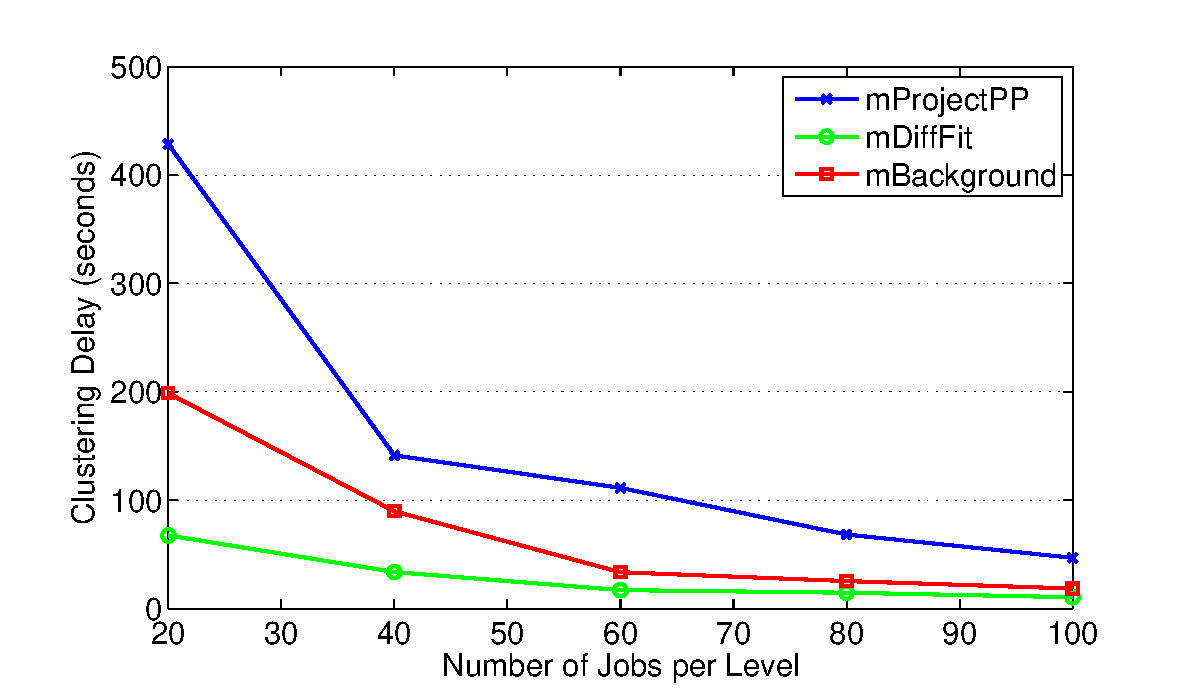
\includegraphics[width=0.9\linewidth]{figures/model/montage_clustering_delay.eps}
    \caption{Clustering Delay of mProjectPP, mDiffFit, and mBackground}
    \label{fig:model_montage_clustering}
\end{figure}





Figure~\ref{fig:model_montage_clustering} shows the average value of Clustering Delay of mProjectPP, mDiffFit, and mBackground. It is clear that with the increase of $k$ (the maximum number of jobs per horizontal level), since there are less and less tasks in a clustered job, the Clustering Delay for each job decreases. For simplicity, we use an inverse proportional model in Equation~\ref{eq:model_clustering_delay} to describe this trend of Clustering Delay with $k$. Intuitively we assume that the average delay per task in a clustered job is constant ($n$ is the number of tasks in a horizontal level). An inverse proportional model can estimate the delay when $k=i$ directly if we have known the delay when $k=j$. Therefore we can predict all the clustering cases as long as we have gathered one clustering case. 

\begin{equation} \label{eq:model_clustering_delay}
\frac{Clustering Delay|_{k=i}}{Clustering Delay|_{k=j}}=\frac{n/i}{n/j}=\frac{j}{i}
\end{equation}




